\subsection{Hagen-Poiseuille Flow}

In the previous test case the channel walls were aligned parallel to the simulation grid. Hence, no further interpolation procedures
are necessary to mimic the exact boundaries.
In order to test the accuracy of the Volume-Fraction and the Interpolation method, a test case with a curved geometry is necessary.
Furthermore this gives the possibility to investigate the error of non-interpolating methods on curved surfaces.
A simple adaption of the planar Poiseuille flow, is the laminar flow through a pipe, also referred to as Hagen-Poiseuille flow \citep{tritton88}.
The setup of the fluid domain is schematically shown in Fig. \ref{validation:setup_hpflow}.

It consist of a circular pipe with the radius $r$, which extends infinitely, parallel to the $x$ axis.
This is realized by using periodic boundaries in $x$-direction.
The center of the pipe is set to $(y, z) = (l_y/2, l_z/2)$.
The velocity profile is a result from a predefined spatial constant pressure gradient $\nicefrac{\partial p}{\partial x}$.
in x-direction, that is added into the Navier-Stokes equation.


\begin{figure}[!bp]
      \centering
        \resizebox{0.7 \textwidth}{!}{
       \import{gfx/immersed_boundary/hpflow///}{setup.pdf_tex}
      }
      \caption{Hagen-Poiseuille flow setup.
                \label{validation:setup_hpflow}
      }
\end{figure}

For an analytical solution of this problem we referr to \citep{Kundu2012}.
Once again a steady state flow can be assumed, which implies $\partial v_z/\partial t = 0$. With the introduction of cylindrical coordinates $(r, \phi, x)$
and the assumption that the flow is independent of $\phi$ the equation of motion reduces to
\begin{align}
    \label{vali:hpflow:navstok}
        0 &= - \frac{\partial p}{\partial x}  +  \frac{1}{\Rey} \frac{1}{r}\frac{\partial}{\partial r}\left(r\frac{\partial u}{\partial r}\right)
\end{align}
where $Re = \nicefrac{V_{m}\Delta h}{\nu}$
and the non-dimenzionalization is given by the scales
    $r^* = \nicefrac{r}{\Delta h}$, $v^*=\nicefrac{V_(\text{m})}{\Delta h}$,
    $t^* = \nicefrac{V_{\text{m}}}{\Delta h}$ and $p^* = p \rho V_{\text{max}}^2$.
The integration of Eq. \ref{vali:hpflow:navstok} gives
\begin{align}
    u &= \frac{r^2}{4\nu}\frac{\partial p}{\partial x} + A \ln r + B
\end{align}

\clearpage
With the use of the boundarie conditions $u(r_0) = 0$ this expression simplifies further to

\begin{align}
    u &= \frac{r^2 - r_0^2}{4}\frac{\partial p}{\partial x}Re
\end{align}
Since $v_{max} \stackrel{!}{=} 1$ by definition, the pressure condition for the domain needs to be set to
\begin{align}
    \frac{\partial p}{\partial x} = -\frac{4 r_o^2}{Re}
\end{align}

\subsection{Simulations}

\subsubsection{Grid Convergence Study with comparsion to the Theoretical Solution}

For an error evaluation a grid convergence study was performed with the Reynolds number set to $Re=100$.
The number of grid points was varied in the intervall $N\in[32, 256]$ furthermore a
simulation with a resolution of $N=512$ was carried out.
Since the maximum velocity of the channel is given by $v_{max}=1$, due to the choice of non-dimensionalization,
the sound speed was set to $c^2 = 100$ to fullfill the incompressibilty condition $Ma = v/c < 0.1$.
The resulting timestep for the highest resolution is $\Delta t = 1e-4$.
The main parameters of the simulation are  given by

\begin{center}
\vspace*{0.7ex}
\begin{tabular}{c|c|c|c|c|c|c }
 $ N  $                   & $\Delta t$ & $\Delta x$            & $\Rey$  & $c^2$   & $l_x, l_y, l_z$ & $T_{end}$\\
\hline
 $[8, 256], \Delta N = 8 $& $10^{-4}$ & $\nicefrac{1}{N - 1}$ & 500     & $500$   & (1, 1, 1)       & 10\\
\end{tabular}
\vspace*{0.7ex}
\end{center}

With this setup all immersed boundary methods were tested for 2nd and 4th order finite difference schemes.\\
For the penalization method the non-dimensionalized damping was set to $J=10^{-4}$.
It would be possible to choose a larger time step for the lower resolution cases, which means that in general
one would apply a smaller damping rate $J$ in a case of an applicaton. To remain consistent in the error convergence, here $J$ and
therefore $\Delta t$ are not altered.

\subsubsection{Long-Term Simulations}

In Order to test the  numerical stability and conservation of mass, a long-term simulation was performed.
A Reynolds number of $Re=100$ was chosen. The resolution is set to $N=96$ grid points.
The ending time was set to $T_end=100$.
The main parameters of the simulation are  given by

\begin{center}
\vspace*{0.7ex}
\begin{tabular}{c|c|c|c|c|c|c }
 $ N  $                   & $\Delta t$ & $\Delta x$            & $\Rey$  & $c^2$   & $l_x, l_y, l_z$ & $T_{end}$\\
\hline
 $[8, 256], \Delta N = 8 $& $10^{-4}$ & $\nicefrac{1}{N - 1}$ & 500     & $500$   & (1, 1, 1)       & 10\\
\end{tabular}
\vspace*{0.7ex}
\end{center}

With this setup all immersed boundary methods were tested for 2nd and 4th order finite difference schemes.\\
Like in section () the non-dimensionalized damping, for the Volume-Penalization was set to $J=10^{-4}$.

\subsection{Results}

\subsubsection{Grid Convergence Study}

The results of the grid convergence study are shown from Fig. \ref{vali:hp_flow_gc_vp} to Fig. \ref{vali:hp_flow_gc_all}.
For a better overview the results are distributed into four plots,
for all methods (except IP-o4) an approximately linear decrease in the double logarithmic space can be observed.

In Fig. \ref{vali:hp_flow_gc_vp} the relative $l_2$-error is shown for different VP-methods.
For the default VP-method of o2 and o4 the error converges rate is about $\lambda=1.17$,
o4 has a smaller error than o2.
The optional use of the VF-method improves the error converges to about $\lambda=1.65$.
Here the o2 method as a smaller error.
It can be noted that the overall error is smaller ($\approx 10^{-2}$ for $N=100$)
when using the optional VF-method in comparsion to the default VP-method ($\approx2\cdot 10^{-2}$ for $N=100$)

In Fig. \ref{vali:hp_flow_gc_df} the relative $l_2$-error is shown for different DF-methods.
For the default DF-method of o2 and o4 the error convergence rate is about $\lambda=1.2$,
again o4 has a smaller error than o2.
The optional use of the VF-method improves the error convergence to about $\lambda=1.4$,
which is worse in comparison to the VP-method, the o2 method has a smaller error then o4.
The overall error is smaller ($\approx 1.5 \cdot 10^{-2}$ for $N=100$) for the VF-method,
in comparsion to the default DF-method ($\approx2\cdot 10^{-2}$ for $N=100$)


In Fig. \ref{vali:hp_flow_gc_ip} the relative $l_2$-error is shown for different IP-methods.


For the IP-o4 method the decay rate is about $1.4$.
For the IP-o2 and IP-DF-o4 method the errors are identical, the decay rate is about $2.4$
The IP-DF-o4 method is numerically not stable and therefore not shown.
From the interpolation methods the IP-o2 method gives the smallest error  ($\approx 5 \cdot 10^{-5}$ for $N=100$).


Finally Fig. \ref{vali:hp_flow_gc_all} shows the method  with the best convergence
rates from the DF, VP and IP methods in one plot.
In summary it can be said that the overall converges rate of the IP-o2-method is of one order better
than the VP-VF and DF-VF methods. The relative error of the interpolation method ranges
between one and two order of magnitudes below all other methods, depending on the resolution.

\begin{figure}[!bp]
  \begin{minipage}[c]{0.5\textwidth}
      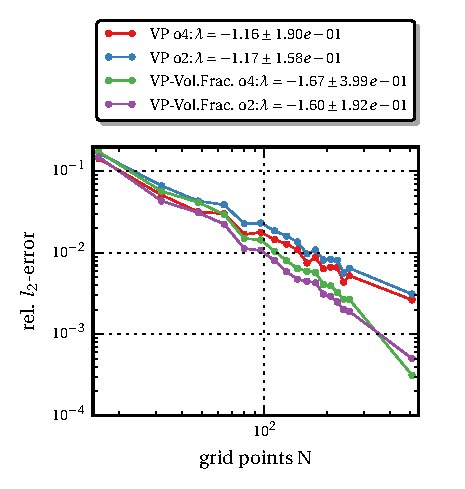
\includegraphics{gfx/immersed_boundary/hpflow/theo/vp.pdf}
      \caption{\label{vali:hp_flow_gc_vp}
          Relative $l_2$-error for different Volume-Penalization methods.}
  \end{minipage}
  \begin{minipage}[c]{0.5\textwidth}
      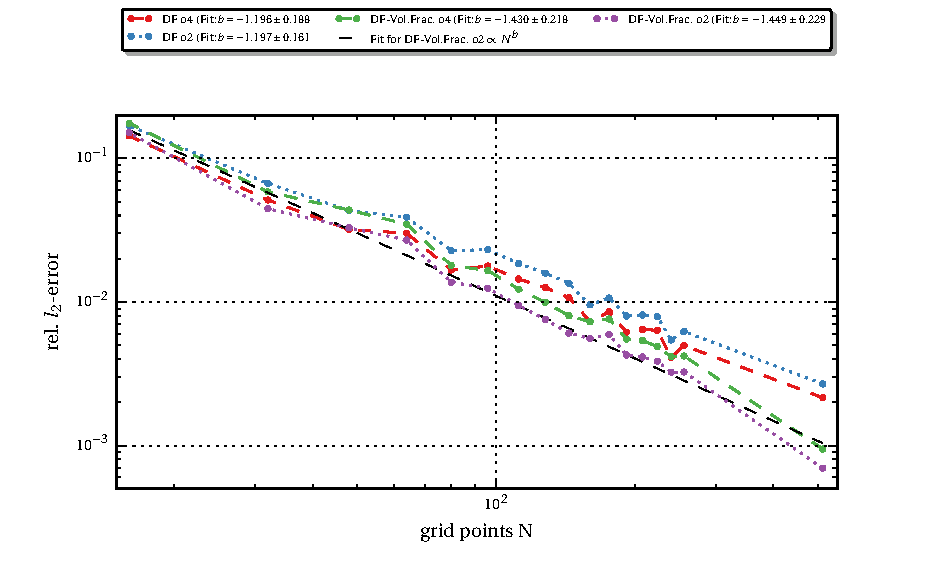
\includegraphics{gfx/immersed_boundary/hpflow/theo/df.pdf}
      \caption{\label{vali:hp_flow_gc_df}
          Relative $l_2$-error for different Direct-Forcing methods.}
  \end{minipage}
  \begin{minipage}[c]{0.5\textwidth}
      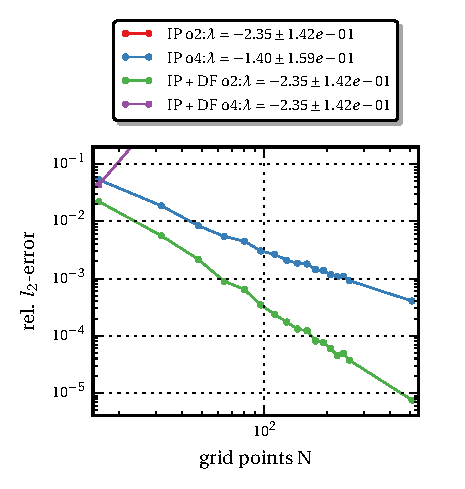
\includegraphics{gfx/immersed_boundary/hpflow/theo/ip.pdf}
      \caption{\label{vali:hp_flow_gc_ip}
          Relative $l_2$-error for different Interpolation methods.}
  \end{minipage}
  \begin{minipage}[c]{0.5\textwidth}
      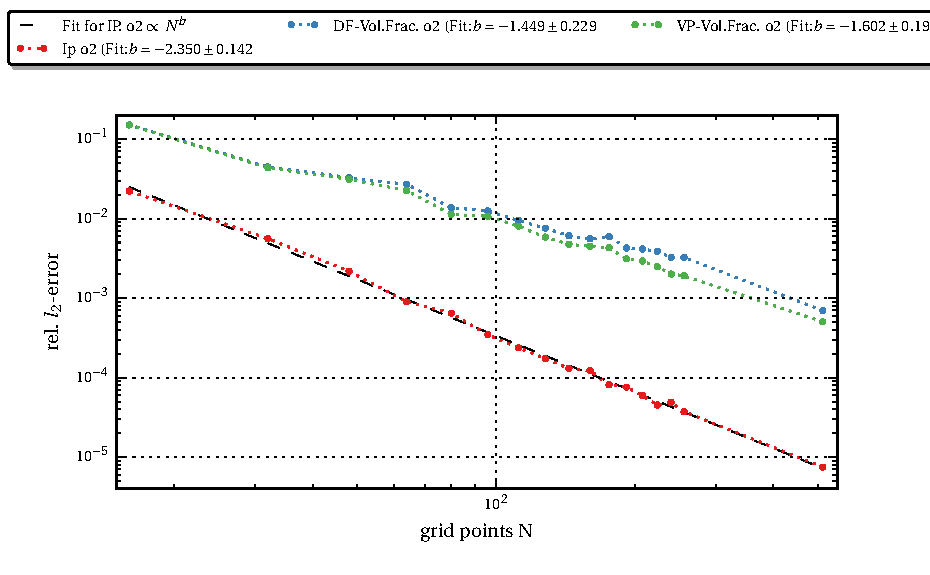
\includegraphics{gfx/immersed_boundary/hpflow/theo/all.pdf}
      \caption{\label{vali:hp_flow_gc_all}
          Relative $l_2$-error for the methods with the smallest error in comparsion.}
  \end{minipage}
\end{figure}

\subsubsection{Long-Term Simulations}

The long-term simulations were performed in order to test the numerical-stability and the conservation of mass.
For all methods, except the IP-o4 method, these simulation were numerically stable.
For all o2 methods, the density averaged of the fluid domain is constant, which indicates that the total mass flux through the
fluid domain boundaries is zero.
It can be seen that for all methods of o4 oscillations in the density emerge.
This is exemplariliy shown in Fig.  \ref{hpflow:results_long_ts} for the DF-VP-o4 method.
The profile of the other o4 methods of is shown in Appendix ().
Finally in Fig. \ref{hpflow:results_long_example} the averaged density with respect to the simulation time is, shown for the
o4 methods.  For the VP and DF methods the density increases to above $5\cdot10^{-5}$.
The VF methods have a decrease in the density, which is remains of the order $10^{-4}$.
For all o4 methods a change in the averaged density followed by a saturation can be observed.

\begin{figure}[tp]
  \begin{minipage}[c]{0.5\textwidth}
      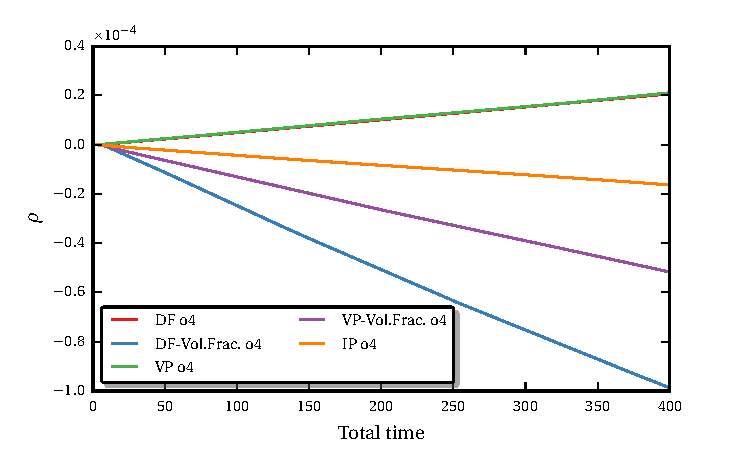
\includegraphics{gfx/immersed_boundary/hpflow/long/ts.pdf}
      \caption{\label{hpflow:results_long_ts}
            Averaged density with respect to the simulation time.
          }
  \end{minipage}
  \begin{minipage}[c]{0.5\textwidth}
      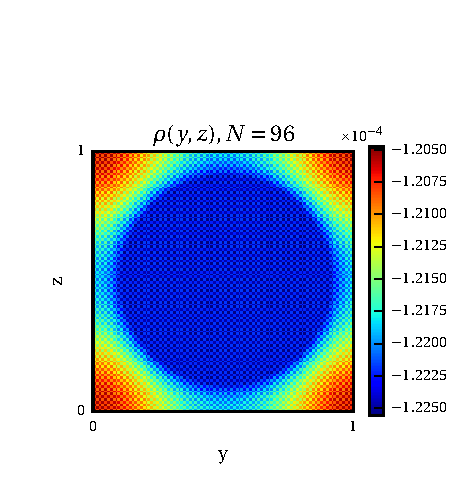
\includegraphics{gfx/immersed_boundary/hpflow/long/example.pdf}
      \caption{\label{hpflow:results_long_example}
        Density in the xy plane for$ z = 0.5 t = tend$.
      }
  \end{minipage}
\end{figure}

\subsection{Discussion}

-all method



-alle methoden except ip haben gleiche fehler ordnung
-fraction methdos is a little bit better
-ip ist am besten mit 2 ordnung

-the best error is interpolation

- ip o4 unstable mit mit DF o4 possible explanation is given in sec. .
- density reaches over the simulation domain


- warum ist ip unstable ???
- ip o2 identical to o4


 The identy of these methods occurs due to the decoupling of the velocity fields
on the border ot the fluid domain. Since the interpolation stencil seperates the fluid and wall domain, the 2nd order
stencil doesn't see any points in the wall domain, therefore there is no difference in using the direct forcing method.\\

\subsubsection{Long-Term Simulations}
- density changes
- interpolation at the boarders
- a part goes into immersed boundar
- howerver the overall influence can be neglected
- explanation decoupling of the pressure


